% posit_pamphlet.tex -- The Posit Pamphlet
% A shirt-pocket reference for posit arithmetic.
%
% Tri-fold layout: 6 panels on US Letter, landscape.
% Fold order (facing you, unfolded):
%   [P6 back-cover] [P1 front-cover] [P2] | [P3] [P4] [P5]
%   left third        center           right of back
%
% Print double-sided, fold in thirds.
%
% pdflatex posit_pamphlet.tex
%
% 2026-11-18  pds/claude

\documentclass[10pt]{article}
\usepackage[landscape, letterpaper,
            top=0.4in, bottom=0.4in,
            left=0.35in, right=0.35in]{geometry}
\usepackage{multicol}
\usepackage{microtype}
\usepackage{booktabs}
\usepackage{array}
\usepackage{amsmath}
\usepackage{amssymb}
\usepackage{parskip}
\usepackage{titlesec}
\usepackage{mdframed}
\usepackage[T1]{fontenc}
\usepackage{lmodern}         % swap for a nicer font when ready
\usepackage[utf8]{inputenc}
\usepackage{wasysym}         % \eighthnote, \quarternote
\usepackage{tikz}
\usetikzlibrary{arrows.meta}

% column rule
\setlength{\columnseprule}{0.3pt}
\setlength{\columnsep}{0.3in}

% tighten section headings
\titlespacing{\section}{0pt}{4pt}{2pt}
\titleformat{\section}{\normalfont\bfseries\small}{}{0em}{}[\titlerule]

% no page numbers
\pagestyle{empty}

% convenience: monospaced box for code snippets
\newenvironment{bitbox}{%
  \begin{mdframed}[linewidth=0.4pt,innerleftmargin=4pt,
                   innerrightmargin=4pt,innertopmargin=3pt,
                   innerbottommargin=3pt]%
  \ttfamily\small\obeylines\obeyspaces
}{%
  \end{mdframed}%
}

% ---------------------------------------------------------------
\begin{document}
\begin{multicols}{3}

% ============================================================
% PANEL 1 -- FRONT COVER / QUICK REFERENCE
% ============================================================
\begin{center}
  {\Large\bfseries The Posit Pamphlet}\\[3pt]
  {\small\itshape perfect arithmetic $\cdot$ pds/claude $\cdot$ 2026}
\end{center}

\section*{Always good to remember}

\smallskip
{\small\ttfamily\noindent\hspace{0.5em}%
k = -(run length)\hfill run of 0s\\[1pt]
\hspace{0.5em}k = \phantom{-(}(run length - 1)\hfill run of 1s}

\vspace{4pt}
{\large
\[
  \text{value} = \text{useed}^k \cdot \left(1 + \frac{f}{2^{\#\text{frac}}}\right)
\]}
\vspace{-10pt}
\[
  \text{useed} = 2^{2^{es}}
\]
\vspace{-6pt}

\noindent\small One rounding, ever.

\section*{Posit4 at a glance}

\begin{center}
\small
\begin{tabular}{rll}
\toprule
value & bits & k \\
\midrule
  0   & 0000 & --- \\
 1/4  & 0001 & $-2$ \\
 1/2  & 0010 & $-1$ \\
 3/4  & 0011 & $-1$ \\
  1   & 0100 &  $0$ \\
 3/2  & 0101 &  $0$ \\
  2   & 0110 &  $1$ \\
  4   & 0111 &  $2$ \\
 NaR  & 1000 & --- \\
 $-4$ & 1001 & $-2$ \\
$-$2  & 1010 & $-1$ \\
$-3/2$& 1011 & $-1$ \\
$-1$  & 1100 &  $0$ \\
$-3/4$& 1101 &  $0$ \\
$-1/2$& 1110 &  $1$ \\
$-1/4$& 1111 &  $2$ \\
\bottomrule
\end{tabular}
\end{center}

\smallskip
\noindent\small \textbf{es} (exponent seed bits) controls dynamic range.
Higher es $\to$ wider range, less precision near 1.
es=0 is the simplest; posit32 es=2 covers all practical needs.

\begin{center}\small
\begin{tabular}{cccc}
\toprule
format & es & useed & quire \\
\midrule
posit4  & 0 &  2 & 16\,b \\
posit8  & 0 &  2 & 32\,b \\
posit16 & 1 &  4 & 64\,b \\
posit32 & 2 & 16 & 128\,b \\
\bottomrule
\end{tabular}
\end{center}

\columnbreak

% ============================================================
% PANEL 2 -- ANATOMY OF IEEE FLOAT
% ============================================================
\section*{Anatomy of IEEE float (32-bit)}

\begin{center}
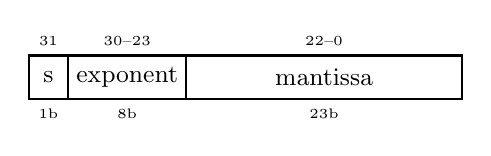
\begin{tikzpicture}[x=1.0cm, y=0.55cm]
  % sign=1b, exponent=8b, mantissa=23b
  \draw[thick] (0,0) rectangle (0.5,1);
  \draw[thick] (0.5,0) rectangle (2.0,1);
  \draw[thick] (2.0,0) rectangle (5.5,1);
  \node[font=\small] at (0.25,0.5) {s};
  \node[font=\small] at (1.25,0.5) {exponent};
  \node[font=\small] at (3.75,0.5) {mantissa};
  \node[font=\tiny,below] at (0.25,0)  {1b};
  \node[font=\tiny,below] at (1.25,0)  {8b};
  \node[font=\tiny,below] at (3.75,0)  {23b};
  \node[font=\tiny,above] at (0.25,1)  {31};
  \node[font=\tiny,above] at (1.25,1)  {30--23};
  \node[font=\tiny,above] at (3.75,1)  {22--0};
\end{tikzpicture}
\end{center}

\noindent value $= (-1)^s \cdot 2^{e-127} \cdot (1 + m/2^{23})$

\smallskip
\begin{tabular}{@{}lp{4.8cm}@{}}
\textbf{sign}     & 0 = positive; 1 = negative \\[1pt]
\textbf{exponent} & biased exponent, bias=127; fixed 8 bits always \\[1pt]
\textbf{mantissa} & fractional part; fixed 23 bits always \\
\end{tabular}

\smallskip
\noindent \textbf{The problems:}

\begin{itemize}\setlength\itemsep{1pt}
  \item Exponent field is fixed-width --- precision is \emph{uniform}
        across all magnitudes. Near $10^{-10}$ you get the same number
        of fraction bits as near $10^{10}$.
  \item $\pm\infty$ and NaN are values --- two hard walls at the ends
        of the number line. Overflow is a cliff, not a slope.
  \item Two zeros ($+0$ and $-0$), special subnormal encoding,
        15 NaN bit patterns. Corner cases compound in long pipelines.
  \item Rounding after every operation. Accumulate enough operations
        and rounding drift is real, expensive to analyze, and
        hardware-dependent.
\end{itemize}

\begin{center}\vspace{-2pt}
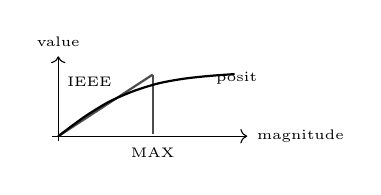
\begin{tikzpicture}[x=0.80cm, y=0.58cm]
  \draw[->] (-0.1,0) -- (3.0,0) node[right, font=\tiny] {magnitude};
  \draw[->] (0,-0.1) -- (0,1.75) node[above, font=\tiny] {value};
  % IEEE: linear then hard cliff
  \draw[thick, gray!60!black] (0,0) -- (1.5,1.35);
  \draw[thick, gray!60!black] (1.5,1.35) -- (1.5,0.05);
  \node[font=\tiny, above left] at (1.0,0.88) {IEEE};
  \node[font=\tiny, below] at (1.5,-0.05) {MAX};
  % posit: tapers asymptotically
  \draw[thick] plot[smooth] coordinates {
    (0,0)(0.4,0.41)(0.8,0.75)(1.2,0.99)(1.6,1.16)(2.0,1.26)(2.4,1.32)(2.8,1.36)
  };
  \node[font=\tiny, right] at (2.35,1.27) {posit};
\end{tikzpicture}
\vspace{-5pt}
\end{center}

\vspace{2pt}
\noindent \textbf{The number line:}

\begin{center}
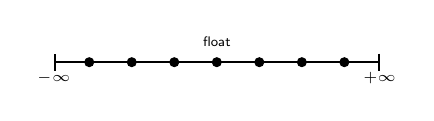
\begin{tikzpicture}[x=0.9cm, y=0.5cm]
  \draw[{Bar}-{Bar}, thick] (-2.3,0) -- (2.3,0);
  \foreach \x in {-1.8,-1.2,-0.6,0,0.6,1.2,1.8}
    \filldraw (\x,0) circle (1.6pt);
  \node[below, font=\tiny] at (-2.3,0) {$-\infty$};
  \node[below, font=\tiny] at ( 2.3,0) {$+\infty$};
  \node[above, font=\tiny] at (0,0.15) {\textsf{float}};
\end{tikzpicture}
\end{center}

Uniform dots. Hard walls at $\pm\infty$.
Overflow is binary: in range, or gone.

\vspace{2pt}
\noindent \textbf{In fairness:}

\noindent$\bullet$ Every modern CPU has a hardware FPU --- single-cycle float.\\
$\bullet$ IEEE 754 is a genuine standard: same bits, same result, any machine.\\
$\bullet$ Fifty years of numerical analysis literature assumes it.\\
$\bullet$ Compiler, debugger, and profiler toolchains speak float natively.\\
$\bullet$ Good enough for most engineering work, most of the time.

\columnbreak

% ============================================================
% PANEL 3 -- ANATOMY OF POSIT
% ============================================================
\section*{Anatomy of a posit bit pattern}

\begin{center}
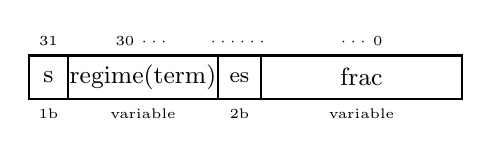
\begin{tikzpicture}[x=1.0cm, y=0.55cm]
  % posit32: sign=1b(31), regime+term=variable(30---), es=2b, frac=variable(---0)
  \draw[thick] (0,0) rectangle (0.5,1);
  \draw[thick] (0.5,0) rectangle (2.4,1);
  \draw[thick] (2.4,0) rectangle (2.95,1);
  \draw[thick] (2.95,0) rectangle (5.5,1);
  % field labels
  \node[font=\small] at (0.25,0.5)   {s};
  \node[font=\small] at (1.45,0.5)   {regime(term)};
  \node[font=\footnotesize] at (2.675,0.5) {es};
  \node[font=\small] at (4.225,0.5)  {frac};
  % bit width below
  \node[font=\tiny,below] at (0.25,0)   {1b};
  \node[font=\tiny,below] at (1.45,0)   {variable};
  \node[font=\tiny,below] at (2.675,0)  {2b};
  \node[font=\tiny,below] at (4.225,0)  {variable};
  % bit numbers above (posit32 reference)
  \node[font=\tiny,above] at (0.25,1)   {31};
  \node[font=\tiny,above] at (1.45,1)   {$30\,\cdots$};
  \node[font=\tiny,above] at (2.675,1)  {$\cdots\cdots$};
  \node[font=\tiny,above] at (4.225,1)  {$\cdots\,0$};
\end{tikzpicture}
\end{center}
\vspace{-4pt}
{\tiny\itshape posit32, es=2; regime boundaries are value-dependent}
\vspace{-2pt}

\begin{tabular}{@{}lp{4.4cm}@{}}
\textbf{sign}   & 0 = positive; 1 = negative (2's complement) \\[1pt]
\textbf{regime} & run of identical bits; 0s $\to$ $k$ negative; 1s $\to$ $k$ positive \\[1pt]
\textbf{term}   & one bit of opposite polarity ends the run; absent when regime fills remaining bits \\[1pt]
\textbf{es}     & exponent seed bits; posit32 has 2; sets $\text{useed}=2^{2^{es}}$ \\[1pt]
\textbf{frac}   & bits after sign, regime, term, es; may be zero \\
\end{tabular}

\smallskip
\noindent \textbf{The regime answers each problem:}

\noindent$\bullet$ Precision follows magnitude --- dense near $\pm 1$, sparse at extremes.\\
$\bullet$ Open ends, no $\pm\infty$. Overflow tapers, never cliffs.\\
$\bullet$ One encoding per value. No $\pm 0$, no subnormals, one NaR.\\
$\bullet$ Quire accumulates exact. One rounding at readout. Drift gone.

\vspace{1pt}
\noindent \textbf{The number line:}

\begin{center}
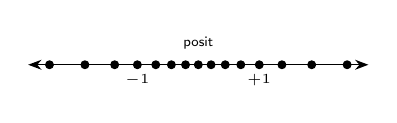
\begin{tikzpicture}[x=0.9cm, y=0.5cm]
  \draw[{Stealth}-{Stealth}, thin] (-2.4,0) -- (2.4,0);
  \foreach \x in {-0.18,-0.38,-0.60,-0.86,-1.18,-1.60,-2.10}
    \filldraw (\x,0) circle (1.4pt);
  \foreach \x in {0.18,0.38,0.60,0.86,1.18,1.60,2.10}
    \filldraw (\x,0) circle (1.4pt);
  \filldraw (0,0) circle (1.4pt);
  \draw (-0.86,-0.08) -- (-0.86,0.08);
  \draw ( 0.86,-0.08) -- ( 0.86,0.08);
  \node[below, font=\tiny] at (-0.86,0) {$-1$};
  \node[below, font=\tiny] at ( 0.86,0) {$+1$};
  \node[above, font=\tiny] at (0,0.15) {\textsf{posit}};
\end{tikzpicture}
\end{center}

No walls. Dots crowd near $\pm 1$.
Precision tapers gracefully toward the extremes.

\medskip
\section*{The regime breathes}

\begin{center}
\small
\begin{tabular}{rllr}
\toprule
value & regime & frac & rs \\
\midrule
 1/4 & \texttt{0 0 | 1} & none & 3 \\
 1/2 & \texttt{  0 | 1} & 1 bit & 2 \\
 3/4 & \texttt{  0 | 1} & 1 bit & 2 \\
  1  & \texttt{  1 | 0} & 1 bit & 2 $\leftarrow$ max \\
 3/2 & \texttt{  1 | 0} & 1 bit & 2 \\
  2  & \texttt{1 1 | 0} & none & 3 \\
  4  & \texttt{1 1   1} & none & 3 \\
\bottomrule
\end{tabular}
\end{center}

Near $\pm 1$: 2-bit regime, 1 fraction bit --- maximum precision.\\
At the extremes: 3-bit regime, no fraction --- precision tapers.\\
\textbf{The regime breathes with the magnitude. That is the whole mechanism.}

\end{multicols}

% ---------------------------------------------------------------
% PAGE 2 -- back side
% ---------------------------------------------------------------
\newpage
\begin{multicols}{3}

% ============================================================
% PANEL 4 -- THE QUIRE REQUIRES
% ============================================================
\section*{The quire requires}

The quire is a wide exact integer accumulator.
Partial sums accumulate without rounding.
One rounding at readout.

\smallskip
\noindent \textbf{Why it matters:}
\[ \frac{1}{2} + \frac{3}{4} + \frac{3}{4} = 2 \]

\noindent \textbf{Without quire} (round each step):
\begin{center}\vspace{-4pt}
$\tfrac{1}{2}+\tfrac{3}{4}=\tfrac{5}{4}$, not in posit4, rounds to $1$\\[2pt]
$1+\tfrac{3}{4}=\tfrac{7}{4}$, not in posit4, rounds to $\tfrac{3}{2}$\\[2pt]
result: $\tfrac{3}{2}$ \quad WRONG
\end{center}\vspace{-6pt}

\noindent \textbf{With quire} (units of $\tfrac{1}{16}$):
\begin{center}\vspace{-4pt}
quire $= 0 + 8 + 12 + 12 = 32$\\[2pt]
$\tfrac{32}{16} = 2$ \quad CORRECT
\end{center}

\smallskip
For posit4: quire is 16 bits, units of 1/16.\\
In RV32I assembly: \texttt{li t0,0 / addi / addi / addi / srli} ---
\textbf{three ADDs and a shift.}

\medskip
\noindent \textbf{Posit4 quire size = $4n = 16$ bits.}\\
Posit32 quire size = $4 \times 32 = 128$ bits.\\
One rounding, ever. Drift simply does not exist.

\columnbreak

% ============================================================
% PANEL 5 -- WHERE POSIT BELONGS
% ============================================================
\section*{Where posit belongs}
\vspace{2pt}
\begin{mdframed}[linewidth=0.4pt,innerleftmargin=6pt,
                 innerrightmargin=4pt,innertopmargin=5pt,
                 innerbottommargin=5pt]
\texttt{fixfft.c} $\to$ signal path (integers, no floats)\\[4pt]
\texttt{posit\_conf()} $\to$ inference layer (posit lives here)
\end{mdframed}

\noindent The FFT produces magnitude-squared values ---
raw energy per bin, nothing more.
The question \emph{``does this bin belong to the chord?''}
is answered in the inference layer.

\medskip
\noindent \textbf{Use fixed-point (integers) when:}
\begin{itemize}\setlength\itemsep{1pt}
  \item You know your value bounds cold
  \item Single-cycle hardware multiplies required
  \item Signal acquisition (ADC hands you integers --- keep them)
\end{itemize}

\noindent \textbf{Use posit when:}
\begin{itemize}\setlength\itemsep{1pt}
  \item Scoring, ranking, probabilistic weights
  \item Multi-frame accumulation (quire eliminates drift)
  \item Physics-adjacent math: sigmoids, \texttt{erfc}, Chauvenet
  \item 32-bit target, need 64-bit accuracy near 1.0
\end{itemize}

\medskip
\noindent \textbf{Arithmetic format choice is inference-layer policy.}\\
It does not belong in the FFT.

\columnbreak

% ============================================================
% PANEL 6 -- BACK COVER
% ============================================================
\begin{center}
  \vspace*{1.5em}
  {\large\bfseries The Posit Pamphlet}\\[6pt]
  {\small\itshape pds / claude \quad 2026}\\[1.5em]

  {\small
  \textbf{Headers and primitives}\\[3pt]
  \textbf{\texttt{bposit\_quire.h}}\\
  \quad\texttt{posit\_pack() \quad posit\_unpack()}\\
  \quad\texttt{quire\_accum() \quad quire\_round()}\\[3pt]
  \textbf{\texttt{quire32.h}}\\
  \quad\texttt{q32\_add() \quad q32\_to\_posit()}\\[3pt]
  \textbf{\texttt{posit\_trig56.h}}\\
  \quad\texttt{sin\_pi() \quad cos\_pi()}\\[6pt]
  \textbf{Ac-cent-tchu-ate the Posit(ive) \quarternote\eighthnote}\\[3pt]
  \begin{minipage}{0.85\linewidth}
  \ttfamily\footnotesize
  \#include "bposit\_quire.h"\\
  quire\_t q = \{0\};\\
  quire\_accum(\&q, posit\_pack(x));\\
  float r = posit\_unpack(quire\_round(\&q));
  \end{minipage}\\[6pt]
  \textbf{Hello world}\\
  \texttt{\footnotesize lab.riscvthai.org/posits/hello.html}\\[3pt]
  \textbf{Source}\\
  \texttt{\footnotesize github.com/psherman42/posits \quad [fe310]}\\[1em]
  }

  {\footnotesize
  Posit arithmetic: John Gustafson, 2017.\\
  \textit{Beating Floating Point at its Own Game.}\\[4pt]
  RISC-V Open Lab\\
  }

  \vfill
  {\footnotesize\ttfamily lab.riscvthai.org}
\end{center}

\end{multicols}
\end{document}
